\section{Comparison of Gas Costs}
\label{sec:comparison}

Because all operations are performed within the Ethereum Virtual Machine,
the primary cost metric is the overall gas cost.
Thus, the focus is on minimizing the total gas used.
Ideally, the best algorithm will have the lowest maximum, mean, and median
gas costs.
We note that the results here are different from those
in~\cite{EfficientIsqrt} for three reasons:
first, some of the algorithms are different
(and we chose the most recent versions of those found online);
second, we ensure that all input values are unique
(there may have been double counting certain evaluations);
third, different input values were chosen.

\subsection{Data Point Selection}

Any gas cost comparison requires the selection of \texttt{uint256}
values for input.
The values were chosen in this way:

\begin{itemize}
\item all numbers of the form $2^{k}$, $2^{k}-1$, and $2^{k}+1$
    for nonnegative values of $k$;
\item $v-1$, $v$, and $v+1$ for $v = (2^{128}-1)^{2}$
    (these were chosen because of an edge case in the new algorithms);
\item random values chosen according to the
    loguniform distribution~\cite{ScipyLoguniform}
    on $\brackets{1, 2^{256}}$ when the random seed
    is initialized to $0$~\cite{NumpyRandomSeed}.
\end{itemize}

\noindent
The number of random samples were increased until
there were $2048$ unique values.
While it is clear that the particular distribution affects to results,
we believe choosing the input values in this way reduces
the risk of potential bias.
There were a total of $768$ deterministic values chosen
and a total of $1303$ random samples were required to determine
the remaining 1280 values.

In addition to measuring the gas cost,
the result of each integer square root operation was
validated using
Python's integer square root~\cite{PythonIsqrt,PythonIsqrtLink}.
There was no instance in which an algorithm ever produced an incorrect result;
this is, of course, not a proof that 
\prb{} (Listing~\ref{list:prb-newton}),
\OpenZeppelin{} (Listing~\ref{list:oz-newton}), and
\abdk{} (Listing~\ref{list:abdk-newton})
are correct,
but rather that there are no known values where these algorithms fail.

\subsection{Summary Statistics}

A listing of the summary statistics describing the runs
may be found in Tables~\ref{table:gas_costs_1}
and \ref{table:gas_costs_2}.
From here, we see that the algorithm with the smallest
maximum, mean, and median gas costs is \UnrolledThree{}.
Although the standard deviation of \UnrolledThree{} is not the smallest,
it is not particularly large.
We note that standard deviations of
\Uniswap{}, \WhileOne{}, \WhileTwo{}, and \WhileThree{}
are larger than the others, and we look at this more closely below.

\subsection{Detailed Analysis}

We now plan to take a closer look at how the gas cost varies
with the argument.
Plots of the gas costs may be found in Figures~\ref{fig:gas_plots_1}
and \ref{fig:gas_plots_2}.

Aside from \Uniswap{}, \WhileOne{}, \WhileTwo{}, and \WhileThree{},
we see from Figures~\ref{fig:gas_plots_1} and \ref{fig:gas_plots_2}
that the gas costs are relatively constant across argument.
In looking at the algorithms, this is not surprising:
\Uniswap{}, \WhileOne{}, \WhileTwo{}, and \WhileThree{}
all have \texttt{while} loops.
In Figure~\ref{fig:gas_plots_2},
we can also see that small arguments in \While{} algorithms
have lower gas costs than the corresponding \Unrolled{} algorithms.
This is not surprising, given that fewer Newton iterations are required,
and exiting before performing unnecessary operations results in a lower cost.

In order to determine when the \Unrolled{} algorithms outperform
the \While{} algorithms,
we determine which algorithms
have the lowest gas cost for each argument evaluated.
After looking at the gas costs from each algorithm,
we counted the number of times each algorithm was minimal;
the results may be found in Table~\ref{table:minimal_gas_costs}.
Additionally, we plot the instances where certain algorithms
were minimal in Figure~\ref{fig:minimal_gas};
a histogram may be found in Figure~\ref{fig:minimal_gas_hist}.
There does not appear to be a particular pattern
in the value distribution.
The main trend is that
\UnrolledThree{} (Listing~\ref{list:newton-unrolled-3})
consistently performs well across the range of arguments.
The only region where this does not hold is for small arguments,
where other algorithms (\While{}) performed better;
this makes sense because fewer Newton iterations are required.

A more extensive analysis may be found in
Appendix~\ref{app:extended};
the results are similar.

\begin{table}[t]
\centering
\begin{tabular}{|c|
    |S[table-format=5.0]|S[table-format=3.0]
    |S[table-format=4.0]|S[table-format=3.0]
    |S[table-format=3.0]|}
\hline
& \Uniswap{} & \prb{} & \OpenZeppelin{} &
    \abdk{} & \python{} \\
\hline
Max    & 34205 & 878 & 1021 & 881 & 963 \\
Mean   & 17734 & 795 &  950 & 803 & 885 \\
Median & 17639 & 798 &  949 & 803 & 888 \\
Std    &  9558 &  34 &   30 &  33 &  44 \\
\hline
\end{tabular}
\caption[Gas Costs Statistics 1]{Here are some statistics
    related to the gas cost data from Figure~\ref{fig:gas_plots_1}.
    We recall that the \Uniswap{} and \python{}
    algorithms are provably correct.
    These results are for the tests in Section~\ref{sec:comparison}.
    }
\label{table:gas_costs_1}
\end{table}

\begin{table}[t]
\centering
\begin{tabular}{|c|
    |S[table-format=3.0]|S[table-format=3.0]
    |S[table-format=3.0]|S[table-format=4.0]
    |S[table-format=4.0]|S[table-format=4.0]|}
\hline
    & \UnrolledOne{} & \UnrolledTwo{} &
    \cellcolor{yellow!25} \UnrolledThree{} &
    \WhileOne{} & \WhileTwo{} & \WhileThree{} \\
\hline
Max    & 858 & 851 & \cellcolor{yellow!25} 831 & 1246 & 1190 & 1177 \\
Mean   & 776 & 775 & \cellcolor{yellow!25} 749 &  853 &  902 &  870 \\
Median & 779 & 777 & \cellcolor{yellow!25} 752 &  898 &  932 &  895 \\
Std    &  42 &  42 & \cellcolor{yellow!25}  41 &  180 &  160 &  141 \\
\hline
\end{tabular}
\caption[Gas Costs Statistics 2]{Here are some statistics
    related to the gas cost data from Figure~\ref{fig:gas_plots_2}.
    We recall that all of these algorithms are provably correct.
    We see that \UnrolledThree{} has the smallest gas costs
    in terms of maximum, mean, and median.
    These results are for the tests in Section~\ref{sec:comparison}.
    }
\label{table:gas_costs_2}
\end{table}

\begin{figure}[p]
\centering
    \begin{subfigure}[t]{0.45\textwidth}
    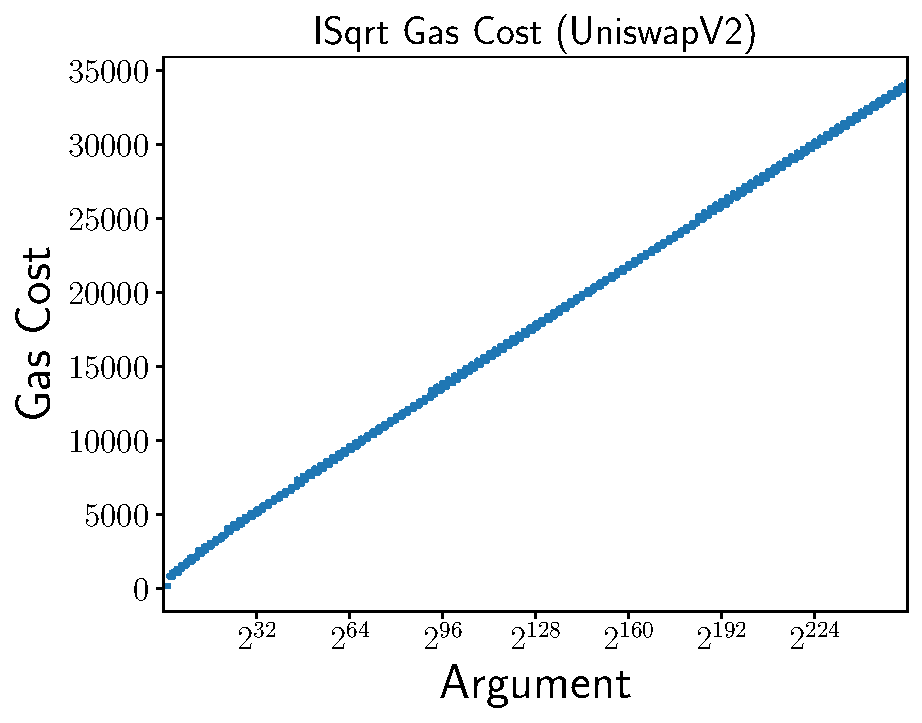
\includegraphics[width=\textwidth]{plots/plot_UniswapV2.pdf}
    \end{subfigure}
    \begin{subfigure}[t]{0.45\textwidth}
    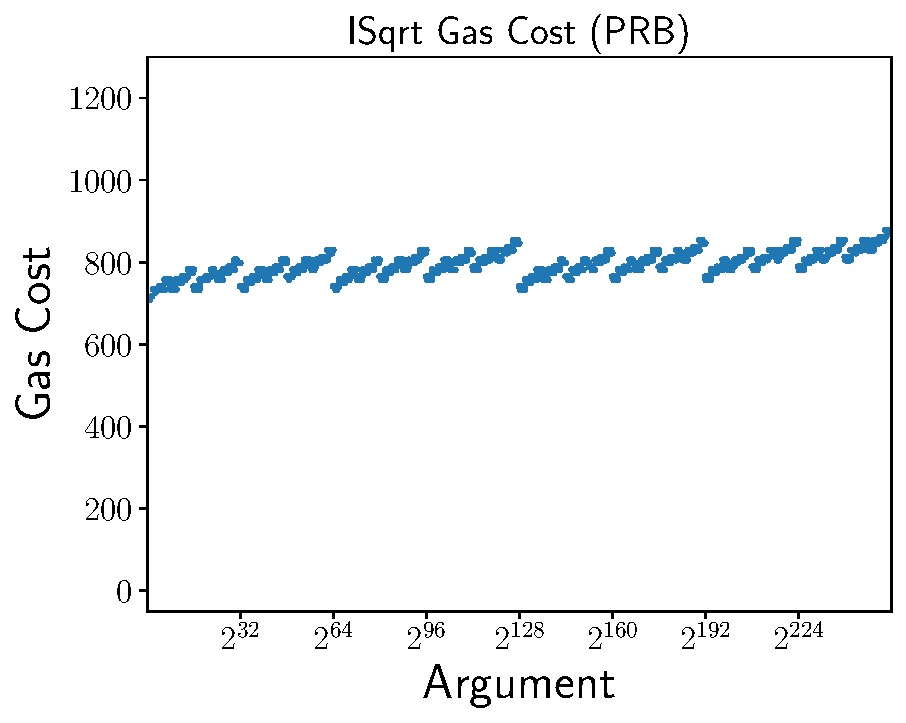
\includegraphics[width=\textwidth]{plots/plot_PRB.pdf}
    \end{subfigure}

    \begin{subfigure}[t]{0.45\textwidth}
    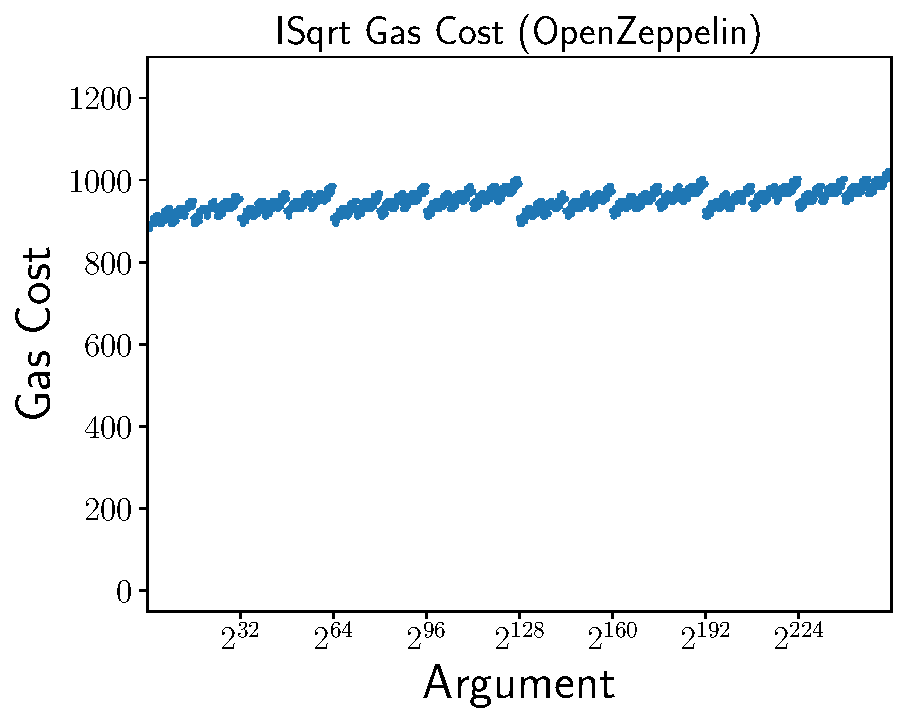
\includegraphics[width=\textwidth]{plots/plot_OpenZeppelin.pdf}
    \end{subfigure}
    \begin{subfigure}[t]{0.45\textwidth}
    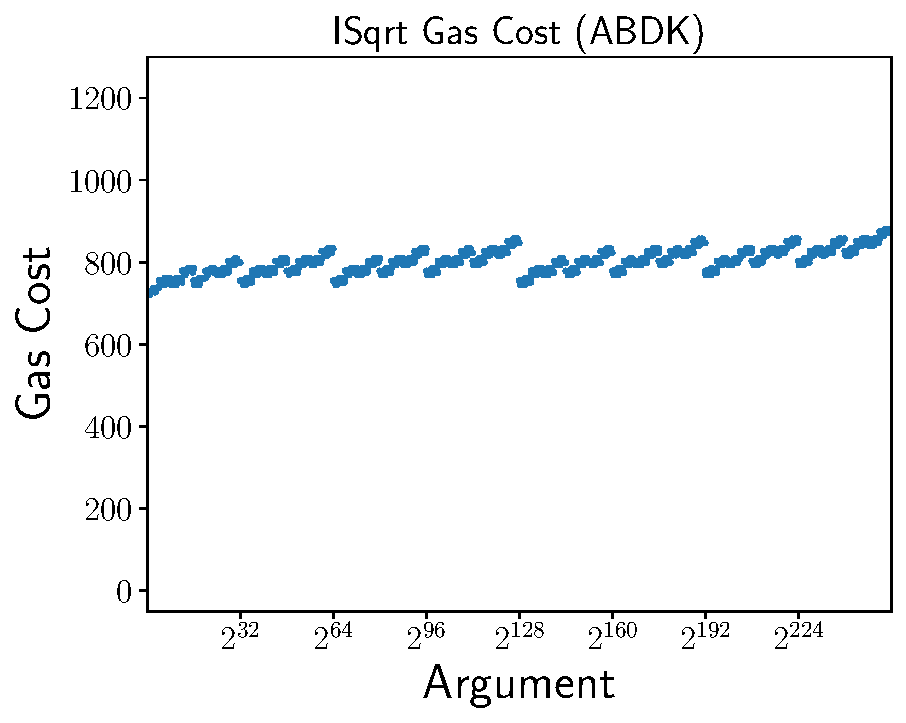
\includegraphics[width=\textwidth]{plots/plot_ABDK.pdf}
    \end{subfigure}

    \begin{subfigure}[t]{0.45\textwidth}
    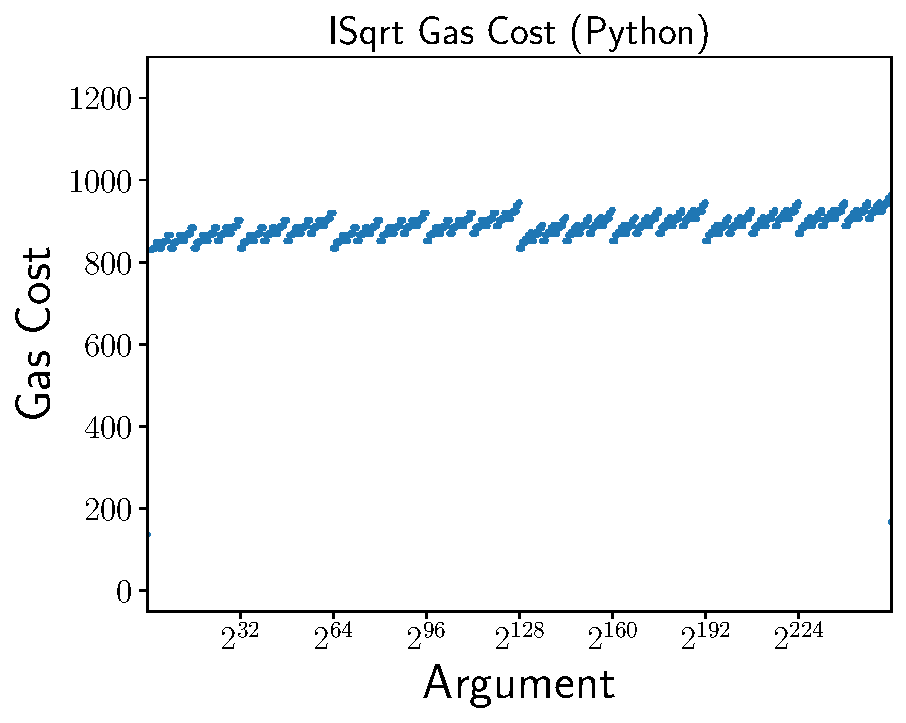
\includegraphics[width=\textwidth]{plots/plot_Python.pdf}
    \end{subfigure}
    \caption{Here are plots of individual gas prices from
        Table~\ref{table:gas_costs_1}.
        Note that all plots except for \Uniswap{} have the same $y$-axis.
        These results are for the tests in Section~\ref{sec:comparison}.
        }
    \label{fig:gas_plots_1}
\end{figure}

\begin{figure}[p]
\centering
    \begin{subfigure}[t]{0.45\textwidth}
    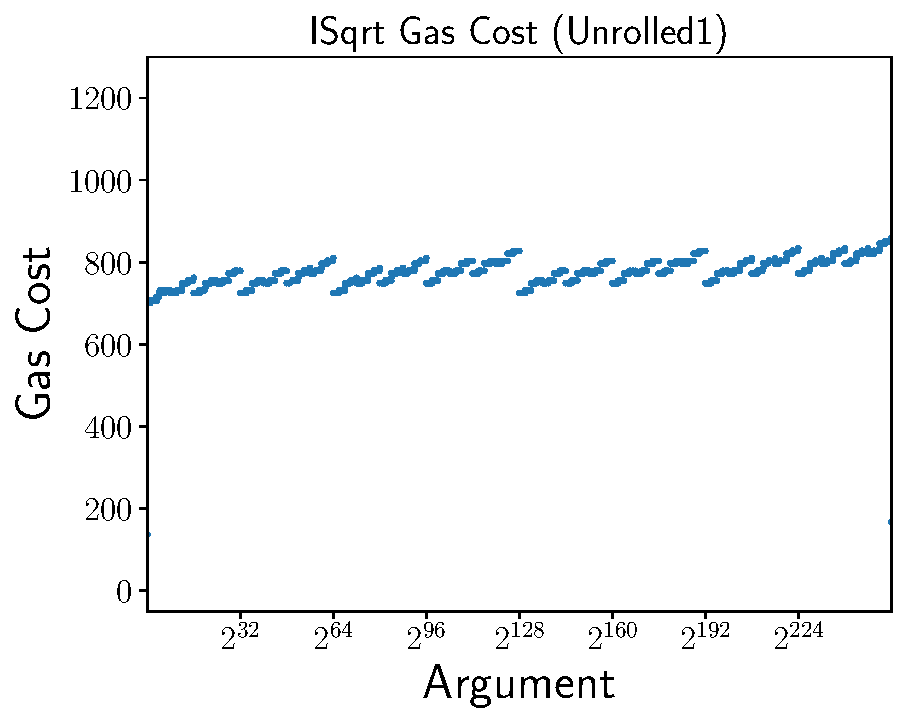
\includegraphics[width=\textwidth]{plots/plot_Unrolled1.pdf}
    \end{subfigure}
    \begin{subfigure}[t]{0.45\textwidth}
    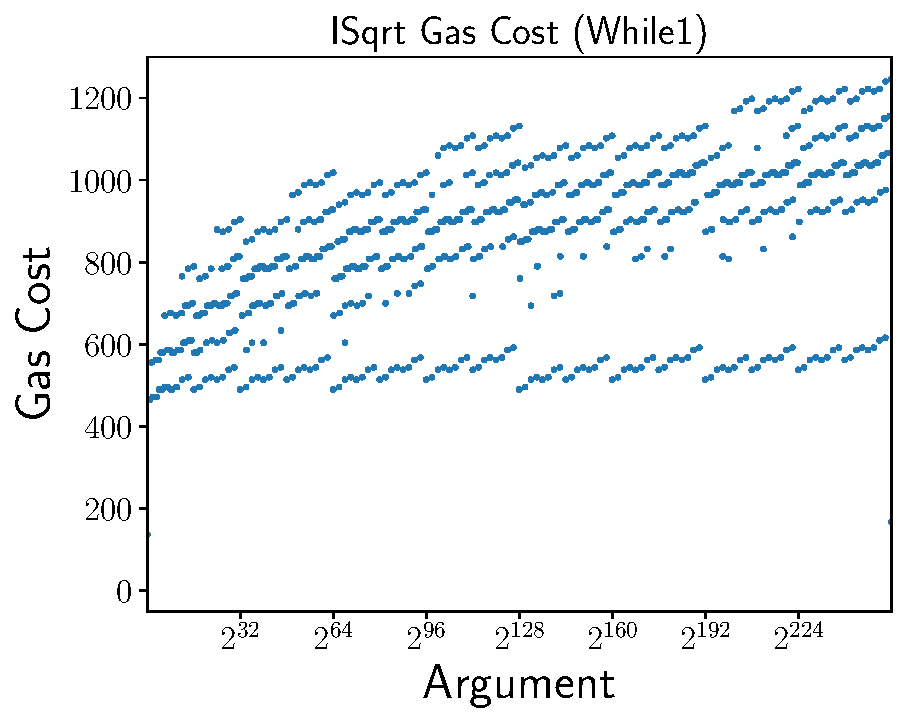
\includegraphics[width=\textwidth]{plots/plot_While1.pdf}
    \end{subfigure}

    \begin{subfigure}[t]{0.45\textwidth}
    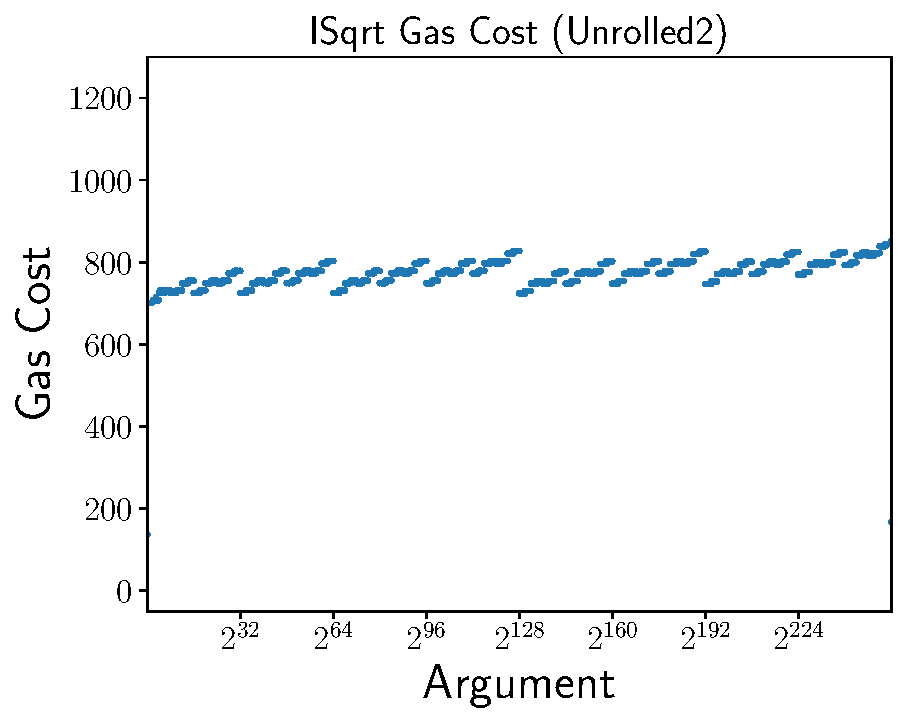
\includegraphics[width=\textwidth]{plots/plot_Unrolled2.pdf}
    \end{subfigure}
    \begin{subfigure}[t]{0.45\textwidth}
    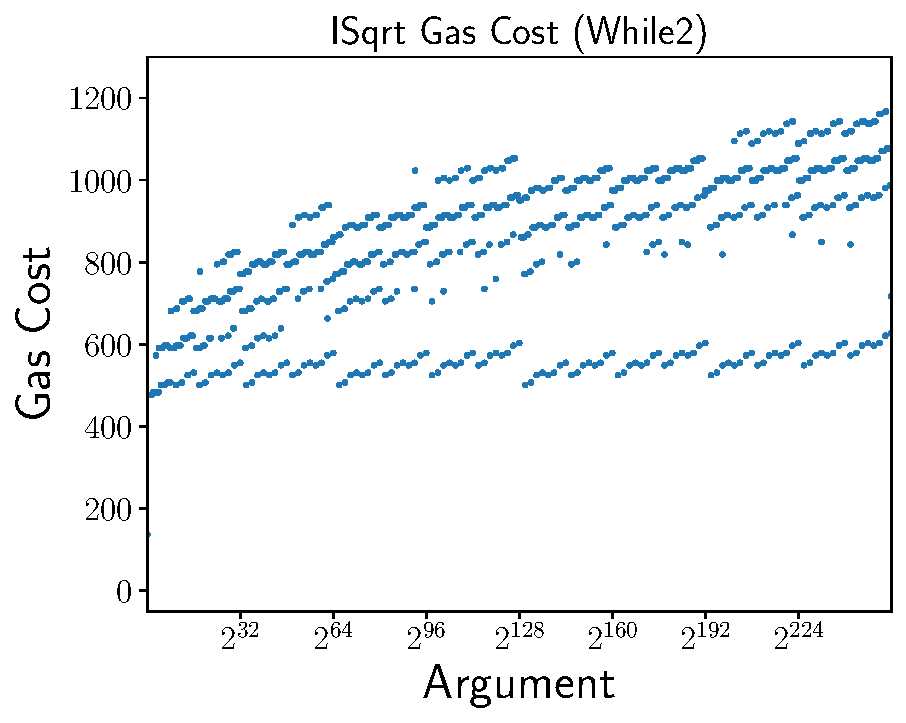
\includegraphics[width=\textwidth]{plots/plot_While2.pdf}
    \end{subfigure}

    \begin{subfigure}[t]{0.45\textwidth}
    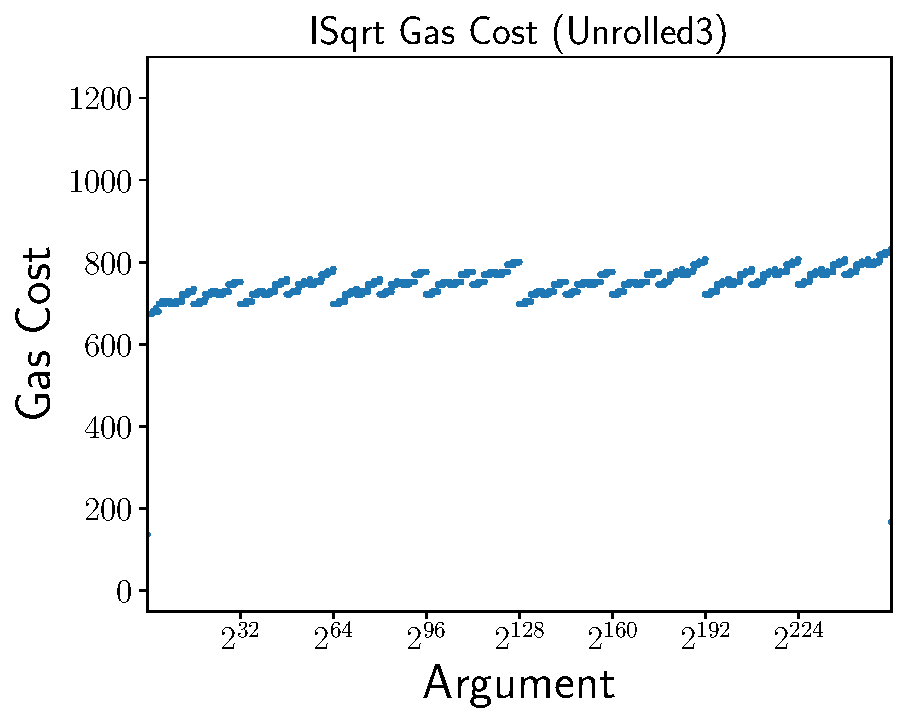
\includegraphics[width=\textwidth]{plots/plot_Unrolled3.pdf}
    \end{subfigure}
    \begin{subfigure}[t]{0.45\textwidth}
    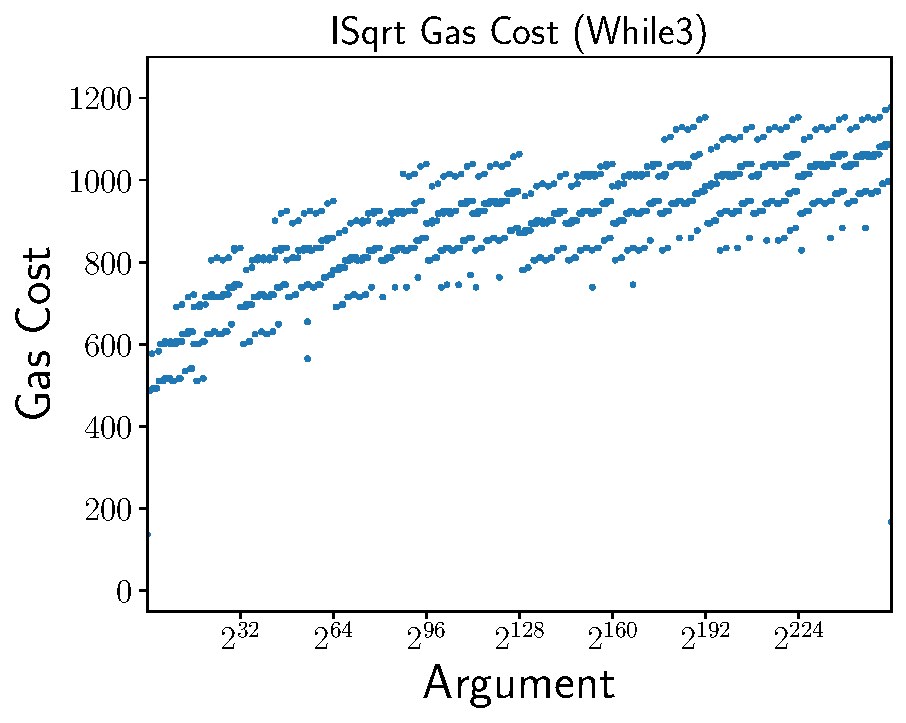
\includegraphics[width=\textwidth]{plots/plot_While3.pdf}
    \end{subfigure}
    \caption{Here are plots of individual gas prices from
        Table~\ref{table:gas_costs_2}.
        All plots have the same $y$-axis.
        These results are for the tests in Section~\ref{sec:comparison}.
        }
    \label{fig:gas_plots_2}
\end{figure}

\begin{table}[p]
\centering
\begin{tabular}{|c|S[table-format=4.0]|}
\hline
Total & 2048 \\
\hline
\Uniswap{}       &    2 \\
\python{}        &    5 \\
\UnrolledOne{}   &    5 \\
\UnrolledTwo{}   &    5 \\
\cellcolor{yellow!25} \UnrolledThree{} & \cellcolor{yellow!25} 1222 \\
\WhileOne{}      &  386 \\
\WhileTwo{}      &  156 \\
\WhileThree{}    &  297 \\
\hline
\end{tabular}
\caption[Minimal Gas Costs Statistics]{Here are number of times
    each method had minimal gas costs;
    methods not included were never minimal.
    These results are for the tests in Section~\ref{sec:comparison}.
    }
\label{table:minimal_gas_costs}
\end{table}

\begin{figure}[p]
\centering
    \begin{subfigure}[t]{0.45\textwidth}
    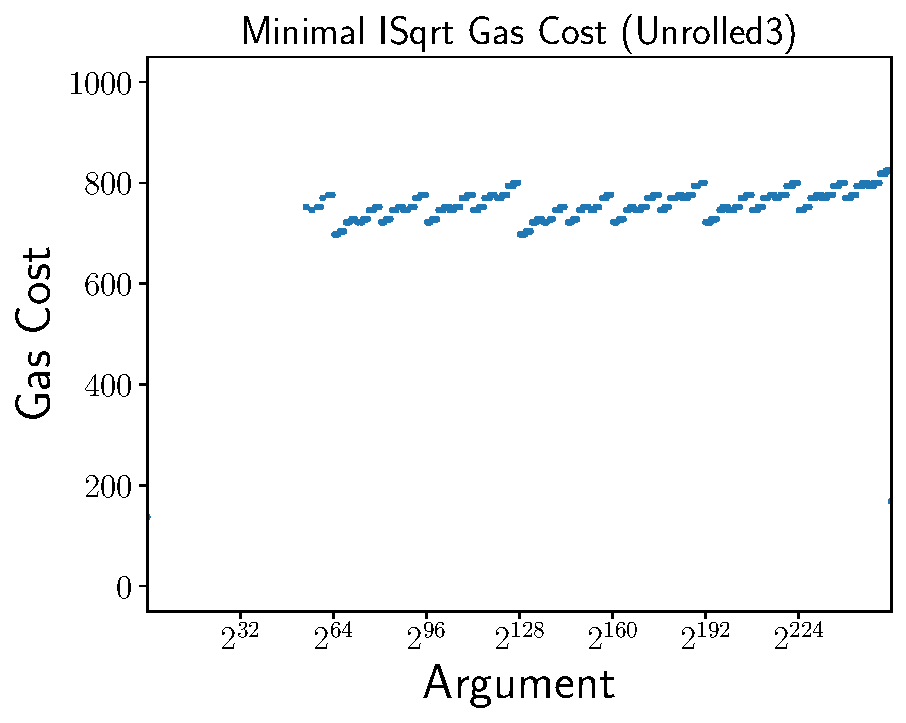
\includegraphics[width=\textwidth]{plots/minimal_plot_Unrolled3.pdf}
    \end{subfigure}
    \begin{subfigure}[t]{0.45\textwidth}
    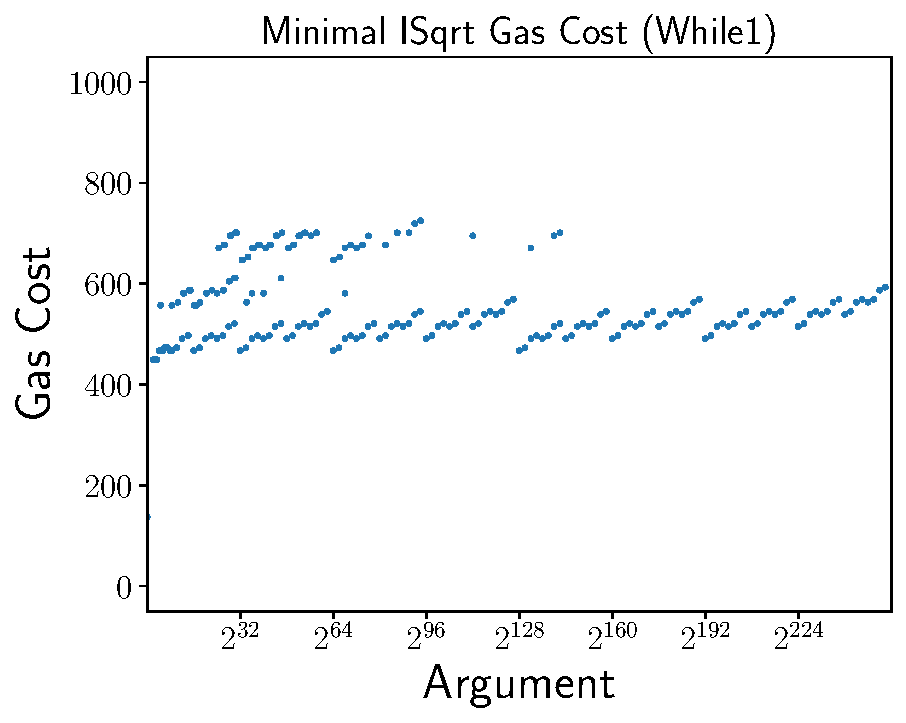
\includegraphics[width=\textwidth]{plots/minimal_plot_While1.pdf}
    \end{subfigure}

    \begin{subfigure}[t]{0.45\textwidth}
    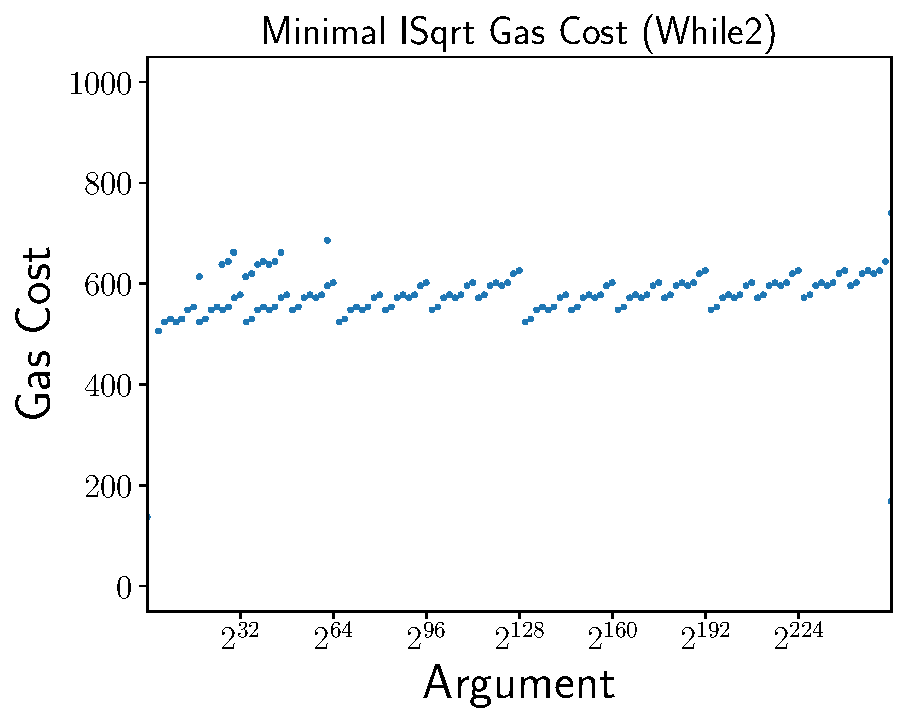
\includegraphics[width=\textwidth]{plots/minimal_plot_While2.pdf}
    \end{subfigure}
    \begin{subfigure}[t]{0.45\textwidth}
    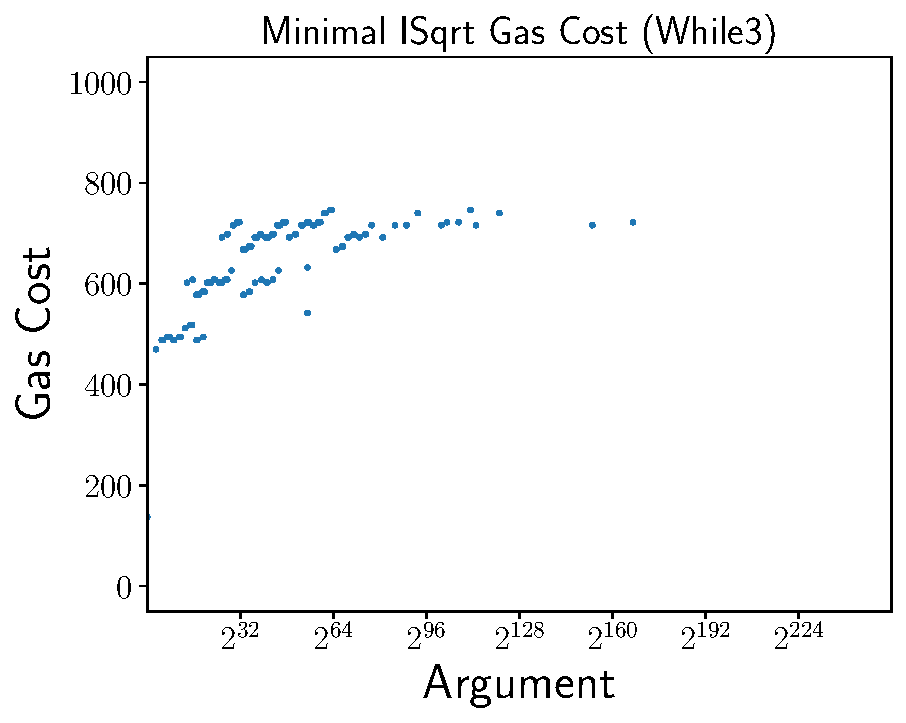
\includegraphics[width=\textwidth]{plots/minimal_plot_While3.pdf}
    \end{subfigure}
    \caption{Here we plot the instances where each algorithm is minimal.
        A histogram of this data may be found in
        Figure~\ref{fig:minimal_gas_hist}.
        These results are the for the tests in Section~\ref{sec:comparison}.
        }
    \label{fig:minimal_gas}
\end{figure}

\begin{figure}[p]
\centering
    \begin{subfigure}[t]{0.45\textwidth}
    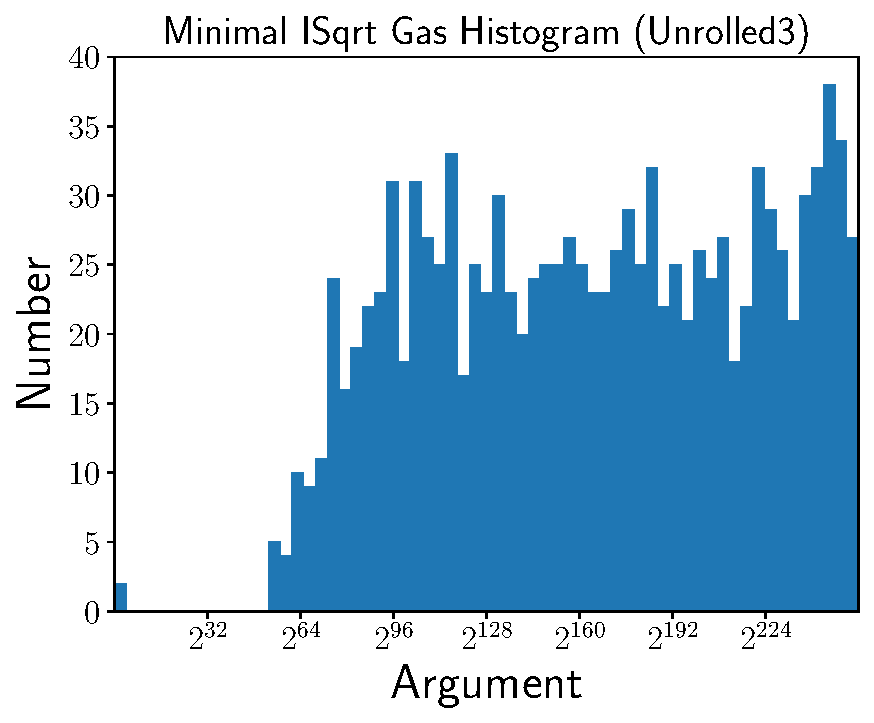
\includegraphics[width=\textwidth]{plots/minimal_hist_Unrolled3.pdf}
    \end{subfigure}
    \begin{subfigure}[t]{0.45\textwidth}
    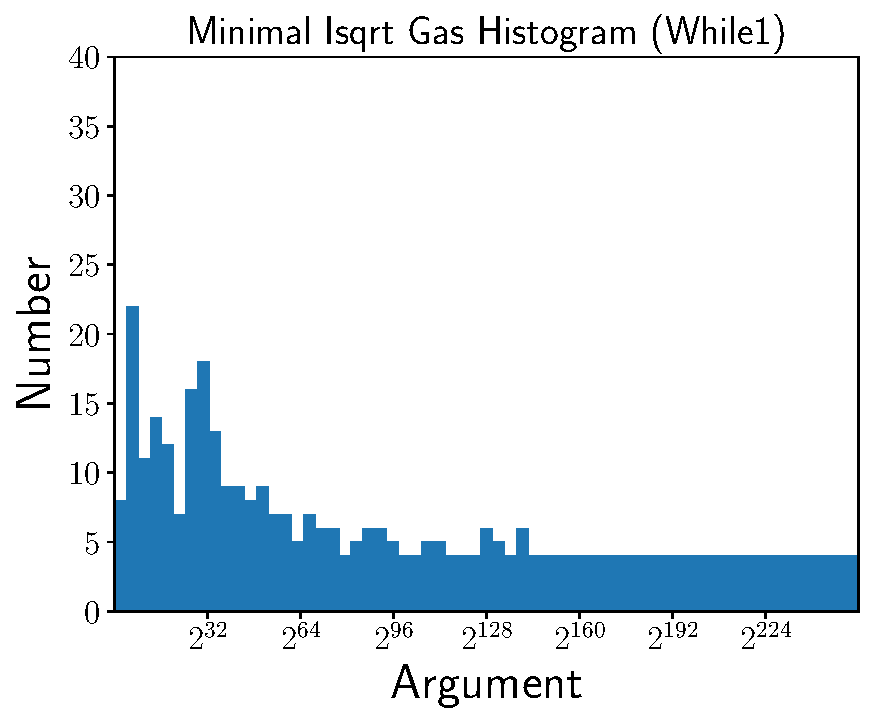
\includegraphics[width=\textwidth]{plots/minimal_hist_While1.pdf}
    \end{subfigure}

    \begin{subfigure}[t]{0.45\textwidth}
    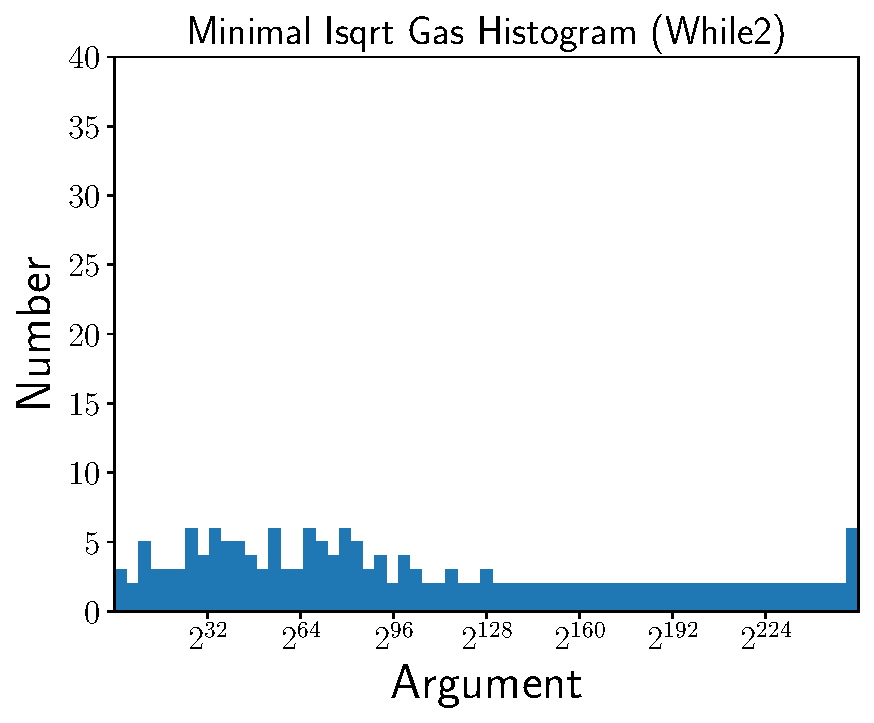
\includegraphics[width=\textwidth]{plots/minimal_hist_While2.pdf}
    \end{subfigure}
    \begin{subfigure}[t]{0.45\textwidth}
    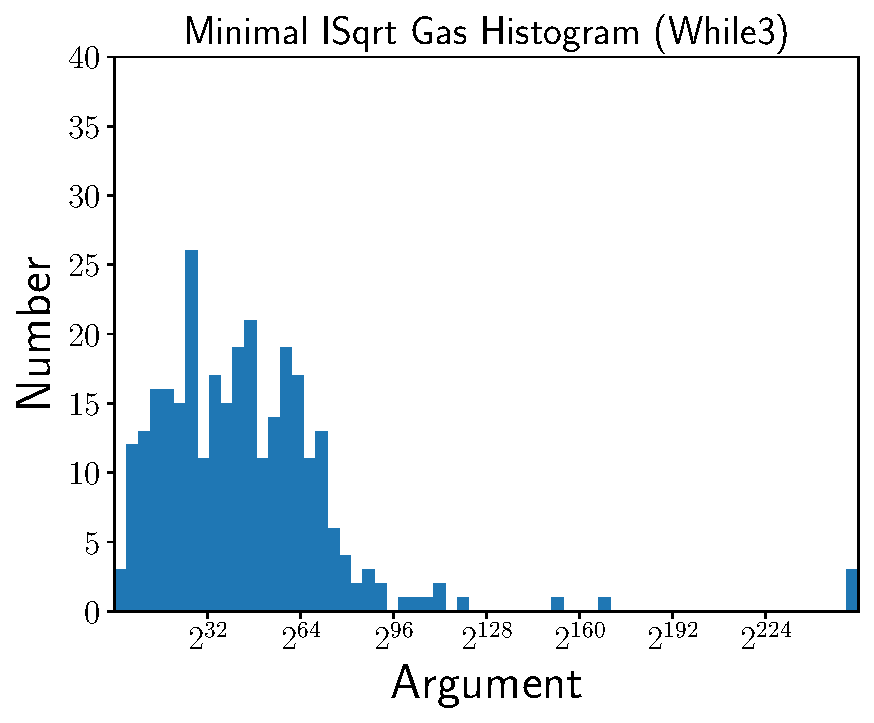
\includegraphics[width=\textwidth]{plots/minimal_hist_While3.pdf}
    \end{subfigure}
    \caption{Here we plot a histogram showing where each algorithm is minimal
        and provides more detail to the results
        in Table~\ref{table:minimal_gas_costs}.
        Each bin counts the total number of instances where the algorithm's
        gas cost is minimal.
        These results are for the tests in Section~\ref{sec:comparison}.
        }
    \label{fig:minimal_gas_hist}
\end{figure}

